\documentclass[11pt,a4paper]{article}
\usepackage[margin=1in]{geometry}
\usepackage{fontspec}
\setmainfont{TeX Gyre Termes}   % Times New Roman look-alike (professional serif)
\usepackage{amsmath,amssymb}
\usepackage{booktabs}
\usepackage{graphicx}
\usepackage{float}
\usepackage{caption}
\usepackage{array}
\usepackage{xcolor}
\usepackage{fancyhdr}
\captionsetup{font=small,labelfont=bf}
\setlength{\parindent}{0pt}
\setlength{\parskip}{6pt}
\pagestyle{fancy}
\fancyhf{}
\rhead{\small\textit{Statistical Analysis of Indian Premier League Match Data}}
\lhead{\small\textit{Case Study}}
\rfoot{\thepage}

\begin{document}

% ------------------------------------------------------------------ TITLE PAGE
\begin{titlepage}
\centering
{
\includegraphics[width=0.28\textwidth]{logo/rajagiri.jpeg}\par}
\vspace{0.8em}
{\LARGE\bfseries Rajagiri College of Social Sciences (Autonomous)\par}
{\large Kalamassery, Kochi, Kerala \par}
\vspace{2.2em}
{\Large\bfseries Statistical Analysis of Indian Premier League Match Data\par}
\vspace{0.6em}
{\large A Case Study in Descriptive Statistics, Probability Modelling and Regression\par}
\vspace{2.5em}
{\normalsize Case Study submitted to Dr.\ Keerthy A. S.\par}
\vspace{3.0em}
{\large\bfseries Submitted by\par}
\vspace{0.8em}
\begin{tabular}{c}
Annsteve Jaison \\[0.25em]
John Jeslin A J \\[0.25em]
Abhishek Vincent
\end{tabular}\par
\vfill
{\normalsize Department of Computer Applications\\ Rajagiri College of Social Sciences (Autonomous), Kalamassery\par}
\vspace{1em}
\end{titlepage}

\pagenumbering{roman}
\tableofcontents
\clearpage
\pagenumbering{arabic}

\section{Introduction}
The Indian Premier League (IPL) is one of the world's most heavily followed
cricket tournaments, and every edition produces a rich
record of match outcomes. The dataset analysed here is derived from the
supplied IPL match archive and records, for every league match, the two
competing teams, the toss, the match venue, the target set by the team batting
first, the manner and margin of victory, and the winner.

\subsection{Dataset and Variables}
The full archive spans 1{,}169 matches from 2008 to 2025. For this study we
restrict attention to the ten-year window \textbf{2008--2018} (seasons 1--11),
yielding 696 matches. After removing 10 abandoned or no-result matches the
working sample contains \textbf{686} decided matches with a single tied match
retained, giving \textbf{10} selected variables drawn from the original 19:

\begin{table}[h!]
\centering
\caption{The ten variables retained for analysis}
\begin{tabular}{lll}
\toprule
\textbf{Variable} & \textbf{Type} & \textbf{Role} \\
\midrule
team1, team2            & Categorical & Competing teams \\
season                  & Discrete     & IPL season code (2008 = 1)\\ 
toss\_winner            & Categorical & Team winning the toss \\
toss\_decision          & Binary       & {\tt bat} or {\tt field} \\
winner                  & Categorical & Match winner \\
venue                   & Categorical & Stadium \\
result                  & Categorical & runs / wickets / tie \\
result\_margin          & Numeric      & Margin of victory (runs or wickets) \\
target\_runs            & Numeric      & Runs set by the first-batting side \\
\bottomrule
\end{tabular}
\end{table}

The objectives are (i) to summarise the population of matches using measures of
central tendency and dispersion; (ii) to model the win process with the
\emph{Binomial} distribution, the focus of the course curriculum; (iii) to model
the wicket-margin variable through its probability mass function and to evaluate
range-based probabilities; and (iv) to test whether first-innings targets have
risen over the decade using simple linear regression.

\section{Descriptive Statistics}
This section summarises the two chief numeric variables: the target set by the
first-batting side (n = 686) and the margin of victory in decided matches
(n = 685; the single tie has no margin).

\subsection{Central Tendency}
For \emph{target runs} the mean is MEAN_TM, the median MED_TM,
and the mode MODE_TM runs. The mean and median are close, indicating that
first-innings targets are broadly symmetric about a typical value near the
160--165 run mark. For \emph{victory margins} the mean is MEAN_MM and the
median only MED_MM; a mean well above the median signals a
distribution dragged upward by a modest number of very large margins.

\subsection{Dispersion}
The standard deviation of targets is SD_TM runs and that of margins
SD_MM runs. Because the two variables differ in scale, the coefficient
of variation is more informative: margins have a coefficient of
variation CV_MM --- more than six times that of targets
(CV_TM). In practical terms, targets are tightly clustered around 160,
whereas match margins are highly volatile.

The quartiles confirm the asymmetry. For targets the interquartile range spans
Q1_TM--Q3_TM (IQR IQR_TM); for margins the IQR spans
Q1_MM--Q3_MM (IQR IQR_MM), with a maximum of
MAX_MM. The skewness of margins is SKEW_MM, strongly positive,
reflecting abundant narrow wins and rare blow-outs. Targets are only mildly
negatively skewed (SKEW_TM).

\begin{figure}[H]
\centering
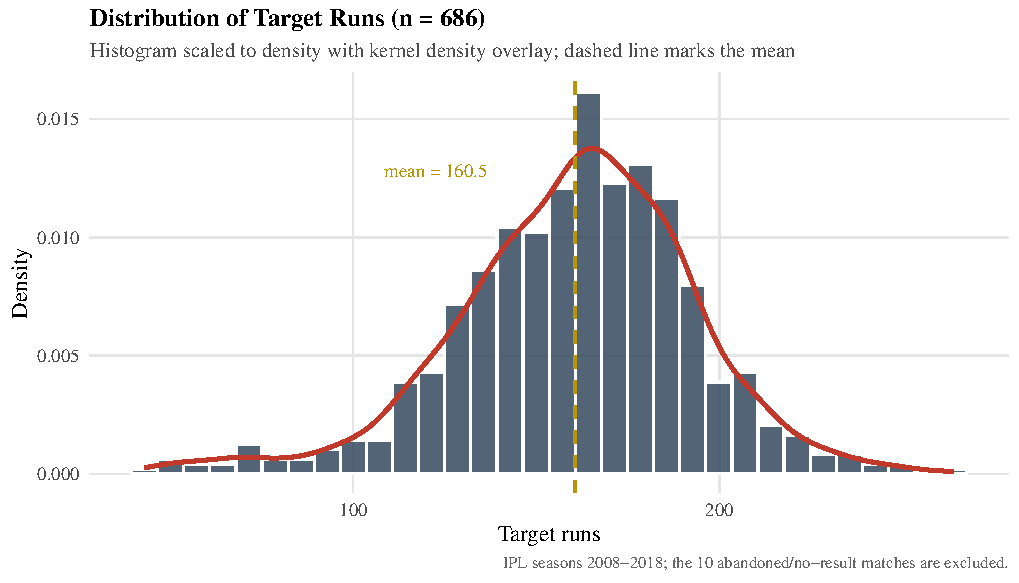
\includegraphics[width=0.92\textwidth]{figures/fig_target_hist.pdf}
\caption{Distribution of first-innings target runs (n = 686). The histogram
is scaled to a density and overlaid with a kernel density estimate; the dashed
line marks the mean of MEAN_TM.}
\end{figure}

\begin{figure}[H]
\centering
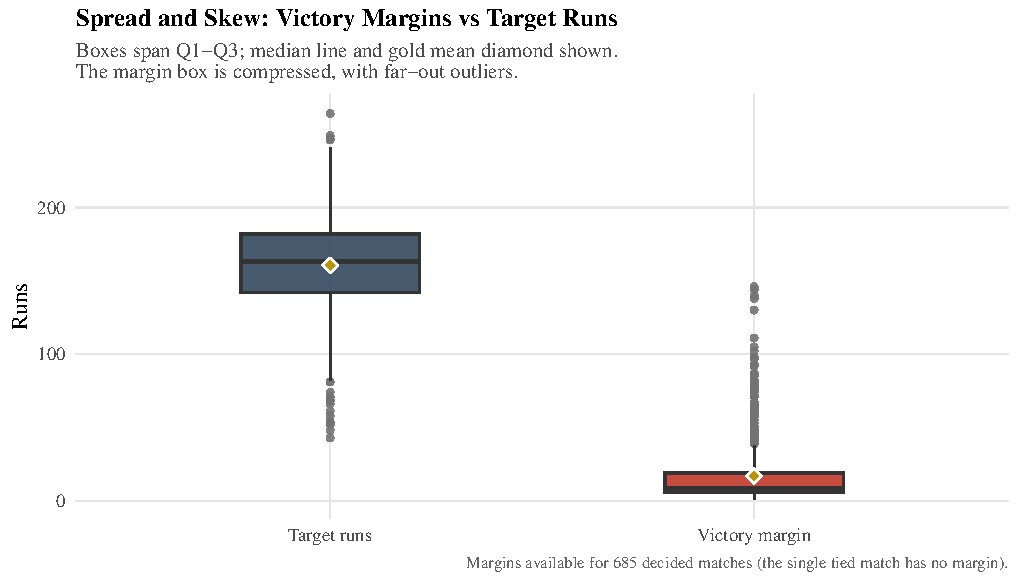
\includegraphics[width=0.92\textwidth]{figures/fig_boxplots.pdf}
\caption{Box-and-whisker comparison of victory margins and target runs. The
compressed margin box with its whisker to MAX_MM illustrates the strong
right skew described in Section 2.2.}
\end{figure}

\section{Probability Modelling}
\subsection{The Binomial Model for First-Innings Advantage}
A natural \emph{Bernoulli} trial is the outcome of a single match, and the
count of wins by a side following a given choice of strategy follows a Binomial
distribution. Let $p$ be the probability that a team which chooses to
\emph{bat first} wins the match. Across the sample, of the
N_BAT matches in which the toss winner chose to bat first,
the same side won K_BAT, giving
$$\hat{p}_{\text{bat}} = \frac{K_BAT}{N_BAT}
= PHAT_BAT.$$
In contrast, of the N_FIELD matches in which the toss winner
chose to field, the chasing side won K_FIELD, so that
$$\hat{p}_{\text{chase}} = PHAT_FIELD.$$

Assuming a fair coin, $p_0 = 0.5$ for either strategy. The exact two-sided
Binomial test of $H_0: p = 0.5$ against $H_1: p \ne 0.5$ yields a
$p$-value of PV_BAT for batting first --- not
significant at $\alpha = 0.05$ --- but PV_FIELD
for chasing, which \emph{is} significant. The 95\% confidence intervals are
$$\text{bat first: }\ [CIB_LO,\ CIB_HI]
\qquad
\text{chasing: }\ [CIF_LO,\ CIF_HI].$$
The chasing interval lies entirely above 0.5, supporting a genuine but modest
first-innings advantage for the fielding side in this era.

\begin{figure}[H]
\centering
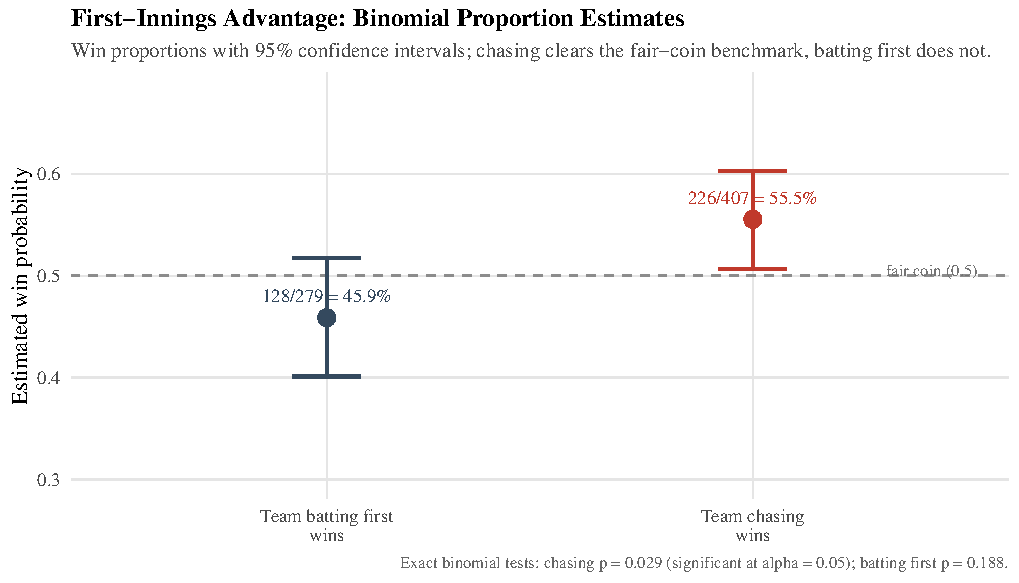
\includegraphics[width=0.9\textwidth]{figures/fig_binomial_ci.pdf}
\caption{Estimated win probabilities under the Binomial model with 95\% Jeffreys
confidence intervals. The chasing estimate clears the fair-coin line; batting
first does not.}
\end{figure}

\subsection{A Probability Mass Function for Wicket Margins}
When a match is won by chasing (n = N_PM), the margin is recorded as the
number of wickets in hand, a discrete variable $X$ taking values from 1 to 10.
Its empirical probability mass function is shown in Figure 3.2; the most likely
outcome is $X = MODE_PM$ with $P(X = MODE_PM) = MAXP_PM$. The
distribution is unimodal and concentrated between 3 and 8 wickets.

\begin{figure}[H]
\centering
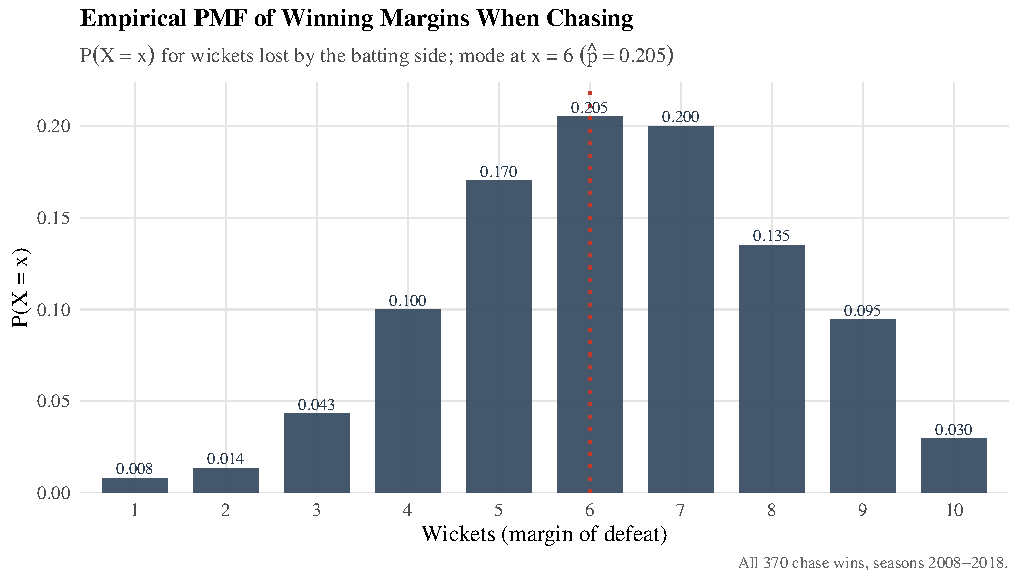
\includegraphics[width=0.9\textwidth]{figures/fig_pmf_wickets.pdf}
\caption{Empirical probability mass function of the wicket margin in the
N_PM chases won by the fielding side.}
\end{figure}

\subsection{Range-Based Probabilities}
Where closed-form integrals of a density are unavailable for empirical data, the
probability of an interval is estimated directly from the relative frequency of
observations in that interval. For target runs $T$:
\begin{align*}
P(140 \le T \le 160) &= P_140_160, &
P(161 \le T \le 190) &= P_161_190, \\
P(T > 200) &= P_GT200, &
P(T < 120) &= P_LT120.
\end{align*}
Nearly P_140_160*100\% of all targets fall in the 140--160 band
and a further P_161_190*100\% in the 161--190 band, so a team
setting a target above 190 enters territory reached in only about
P_GT200*100\% of matches. For victory margins, P(margin $>$ 50) =
P_M50 and P(margin $\ge$ 100) = P_M100,
again illustrating how rare outright domination is relative to close finishes.

\section{Regression Analysis}
To test whether first-innings targets drifted upward over the decade we fit a
simple linear regression of the mean target on season:
$$\hat{y} = a + b\,x,$$
where $x$ is the season code (1--11). Least squares gives
$$\hat{y} = REG_INT + REG_SLP\,x,$$
implying an average increase of REG_SLP runs per season. The fitted
model explains REG_R2*100\% of the variance in seasonal mean targets
($R^2 = REG_R2$), and the slope is significant at the 5\% level
($p = REG_PV$).

\begin{figure}[H]
\centering
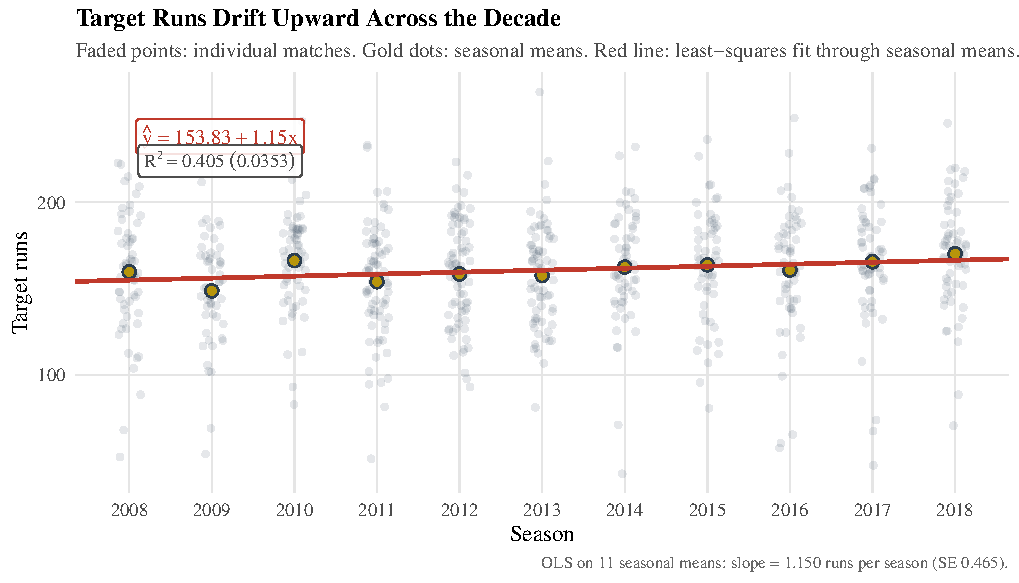
\includegraphics[width=0.92\textwidth]{figures/fig_regression.pdf}
\caption{First-innings target vs season. Individual matches are shown faded, the
gold points are seasonal means, and the red line is the least-squares fit.
The positive slope supports a gradual inflation of scoring across 2008--2018.}
\end{figure}

\section{Conclusion and Reflection}
The analysis paints a coherent picture of a decade of IPL cricket. First-innings
targets are concentrated near 160--165 runs, are mildly left-skewed, and drift
upward by roughly REG_SLP_R1 runs per season --- a statistically
detectable increase in scoring. Match margins, by contrast, are highly
right-skewed: most games are decided by a handful of runs or wickets, while
blow-outs beyond 50 are rare (about P_M50*100\% of decided
matches).

On the probabilistic side, the Binomial model reveals a genuine first-innings
advantage for the chasing side ($\hat{p} = PHAT_FIELD$,
$p = PV_FIELD$), a result consistent with the fielding
advantage under floodlights. Team dominance is real but measured: Chennai Super
Kings won CSK_W of their CSK_G matches
($\hat{p} = CSK_P$, $p = CSK_PV$), a rate the
Binomial test confirms against a fair-coin null, while Mumbai Indians
($\hat{p} = MI_P$) fall just short of conventional significance.

The techniques used --- descriptive statistics, empirical PMFs, range-based
probabilities and the Binomial model --- map directly onto the course curriculum
and are well suited to match-level data. Their principal limitation is that
relative-frequency estimates of probability rest on the assumption that the
sample is representative of the broader population of IPL matches; conclusions
therefore describe the 2008--2018 era rather than cricket in general. A further
limitation is the collapse of many rich covariates (player lists, venues, pitch
conditions) into ten variables; a hierarchical model that respected venue and
opponent strength would refine the estimates, but lies beyond the scope of this
case study.

\end{document}
